\chapter{Potential elastica energy}
\label{chapter:appendix-potential-elastica-energy}

\begin{definition}{Balance coefficent}
Given digital shape $S \in \Omega$, positive number $r$ and point $p \in S$, the \emph{balance coefficient} of $S$ at $p$ is defined as

\begin{align*}
	u(p) = \left( \frac{\pi r^2}{2} - |B_r(p) \cap S| \right)^2.
\end{align*}

\end{definition}

The balance coefficient is a measure of how close an estimation ball is from estimating zero curvature. In figure \ref{fig:balance-plot}, we plot the balance coefficients of points in the diagonal of a square shape. 

\begin{figure}[h!]
\center
\begin{minipage}{0.25\textwidth}
\subfloat{
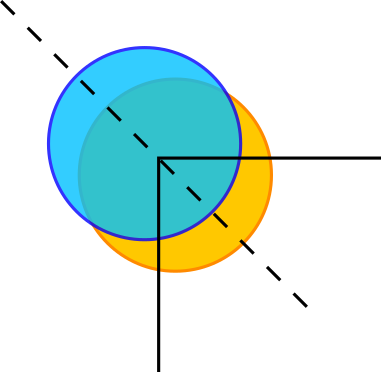
\includegraphics[scale=1.0]{figures/appendix-potential-elastica/distant-disks-1.png}}\\%
\subfloat{
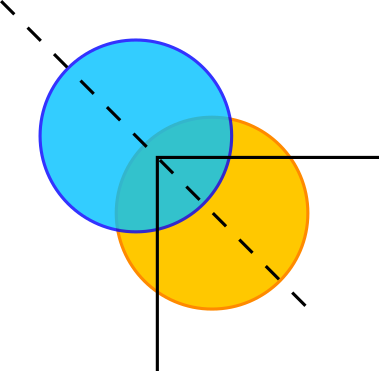
\includegraphics[scale=1.0]{figures/appendix-potential-elastica/distant-disks-2.png}}\\%
\subfloat{
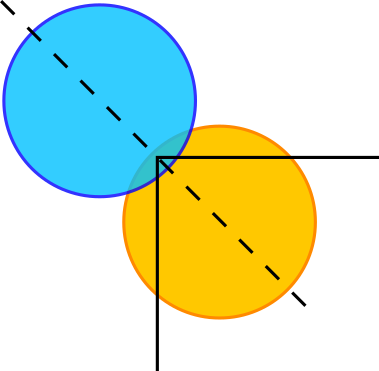
\includegraphics[scale=1.0]{figures/appendix-potential-elastica/distant-disks-3.png}}
\end{minipage}%
\begin{minipage}{0.75\textwidth}
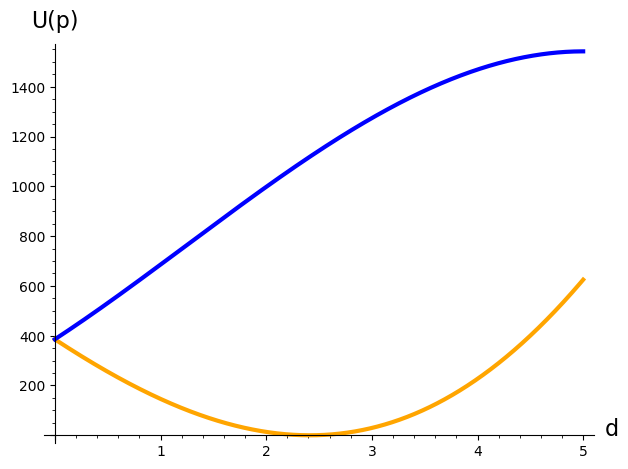
\includegraphics[scale=0.75]{figures/appendix-potential-elastica/potential-elastica-plot.png}
\end{minipage}
\caption{The balance difference of equidistant points from the shape contour preserves squared curvature information.}
\label{fig:balance-plot}
\end{figure}


We notice that difference between outer and inner balance is non-negatice along all the points in the diagonal. In fact, this is true for any point of positive curvature. The difference is negative for points of negative curvature. This is the key observation for the definition of the digital flow.

\begin{definition}{k-potential}
Given digital shape $S$, natural numbers $r>0, k \neq 0$, the \emph{k-potential} at point $p$ is defined as

\begin{align*}
	U_{S,k}(p) &= \sum_{q \in Q(p)}{ u(q),}
\end{align*}

where its balance set $Q(p)$ is defined as

\begin{align*}
	\mathcal{Q}(p) &= \left\{\; q \; | \; q \in L_k(S),\; p \in B_r(q) \; \right\}.
\end{align*}

\end{definition}

\begin{figure}[h!]
\center
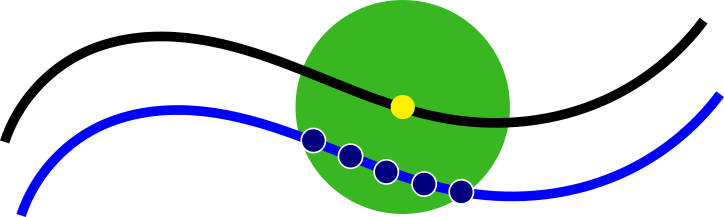
\includegraphics[scale=0.5]{figures/appendix-potential-elastica/k-potential.png}
\caption{The blue points forms the balance set of yellow point.}
\label{fig:balance-set}
\end{figure}

The balance set of $p$ is the set of all points $q$ in which the $p$ is contained in the estimation ball centered at $q$.  In figure \ref{fig:balance-set} we illustrate the balance set definition. The k-potential is used to decide which pixels are to be removed or to be kept in the next shape of the flow. 


\begin{definition}{$k$-flow}
	Given digital shape $X$, we define its $k$-flow as
	
	\begin{align*}
		F_k = \Big\{& X^{(i)} \; | \\
			& X^{(0)} = X,\\
		    &X^{(i+1)} = \argmin \sum_{ x_j \in \mathbbm{1}^{O(X^{(i)})}}{ x_j \Delta _j\big(\; U_{X^{(i)},k}(x_j) - U_{X^{(i)},-k}(x_j) \;\big)} \; \Big\}.
	\end{align*}
     	  
\end{definition}	

\section{Balance plot development}
	The balance difference at a point $c \in S$ distant $d$ units from the corner is written as
	\begin{align*}
		u_i(c) &= \frac{\pi r^2}{2} - \big( \; a^2 + area( APC ) + area(A'PC) + area(\arc{PQ})  \; \big) \\
		&= \frac{\pi r^2}{2} - \big( \; a^2 + a(P_x-a) + \frac{\theta_P + \theta_Q + \pi/2}{2\pi} \pi r^2\; \big),
	\end{align*}
	
	where
	
	\[
	\begin{array}{ll}
	a = d\sqrt{1/2} & \theta_P = \arctan \frac{a}{P_x-a} \\		
	Q_y = -P_x = a + \sqrt{r^2 -a^2} & \theta_Q = \arctan \frac{a}{|Q_y|-a}		
	\end{array}\]
	
%default = pi*R^2*(abs(t2) + abs(phi))/(2*pi) + a*abs(p2[0])

%g2 = pi*R^2/2 - ( pi*R^2 - ( pi*R^2/4 - default) )	
	
	Similarly, for the outer ball
	\begin{align*}
		u_o(c) &= \frac{\pi r^2}{2} - \big(\; \frac{\pi r^2}{4} - area(APC) - area(AQC) - area(\arc{CP'}) - area(\arc{CQ'}) \; \big)\\
		&= \frac{\pi r^2}{2} - \big( \; \frac{\pi r^2}{4} - aP_x - \frac{\theta_P + \theta_Q}{2\pi}\pi r^2 \; \big),
	\end{align*}
	
	where
	\[
	\begin{array}{ll}
		a = d\sqrt{1/2} & \theta_P = \arctan \frac{a}{P_x+a}\\
		Q_y = -P_x = \sqrt{r^2-a^2} - a & \theta_Q = \arctan \frac{a}{|Q_y|+a}
	\end{array}	 \]
	
\begin{figure}[h!]
	\begin{minipage}{0.5\textwidth}
	\center
	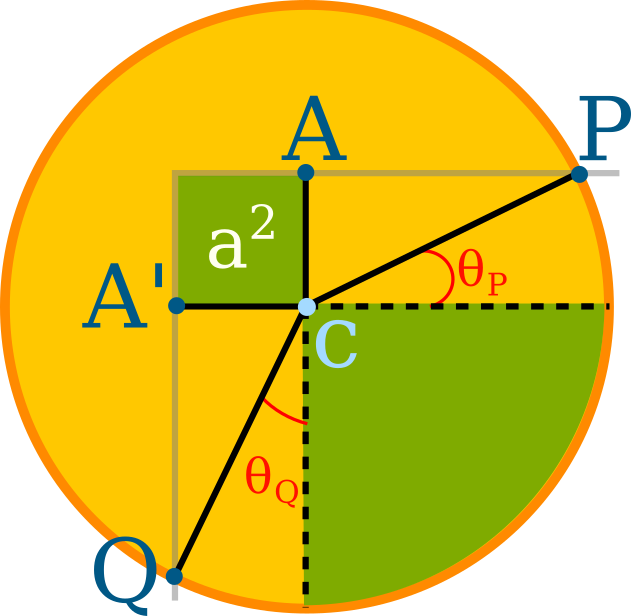
\includegraphics[scale=2.0]{figures/appendix-potential-elastica/balance-dev-1.png}
	\end{minipage}%
	\begin{minipage}{0.5\textwidth}
	\center
	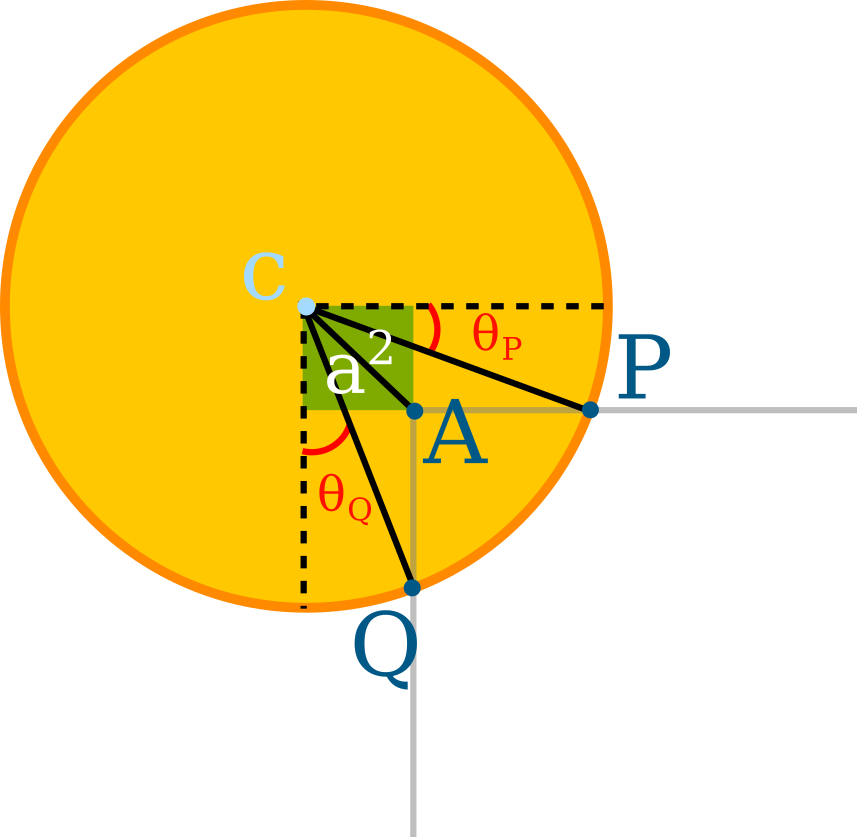
\includegraphics[scale=2.0]{figures/appendix-potential-elastica/balance-dev-2.png}
	\end{minipage}	
\end{figure}

\section{Sage script}

\begin{lstlisting}
var ('d','R')
a=d*sqrt(1/2)

P1x = a+sqrt(R^2-a^2)	#always positive
Q1y = a+sqrt(R^2-a^2)	#always positive

t1 = arctan2(a,P1x-a)
b1 = arctan2(a,Q1y-a)

g1 = pi*R^2/2 - ( a^2 + (P1x-a)*a + pi*R^2*(t1+b1+pi/2)/(2*pi) )


P2x = sqrt(R^2-a^2)-a	#always positive
Q2y = sqrt(R^2-a^2)-a	#always positive

t2 = arctan2(a,P2x+a)
b2 = arctan2(a,Q2y+a)

g2 = pi*R^2/2 - (pi*R^2/4 - P2x*a - pi*R^2*(t2+b2)/(2*pi) )

f = g1^2-g2^2

plot( (g1^2).subs(R=5),(d,0,5),color='orange',thickness=3,axes_labels=['d','U(p)'] ) + plot( (g2^2).subs(R=5),(d,0,5),color='blue',thickness=3)
\end{lstlisting}